\documentclass{article}
\usepackage[utf8]{inputenc}
\usepackage[T1]{fontenc}
\usepackage[english]{babel}
\usepackage{listings}
\usepackage{color}
\usepackage{graphicx}
\usepackage{fullpage}

\usepackage{array,multirow,makecell}
\setcellgapes{1pt}
\makegapedcells
\usepackage[table]{xcolor}

\newcommand{\HRule}{\rule{\linewidth}{0.5mm}}

\lstset{
  backgroundcolor=\color{white},
  basicstyle=\footnotesize,
  breakatwhitespace=false,
  breaklines=true,
  captionpos=b,
  commentstyle=\color{red},
  deletekeywords={...},
  escapeinside={\%*}{*)},
  extendedchars=true,
  frame=false,
  keepspaces=true,
  keywordstyle=\color{blue},
  language=Java,
  literate=
  {²}{{\textsuperscript{2}}}1
  {⁴}{{\textsuperscript{4}}}1
  {⁶}{{\textsuperscript{6}}}1
  {⁸}{{\textsuperscript{8}}}1
  {€}{{\euro{}}}1
  {é}{{\'e}}1
  {è}{{\`{e}}}1
  {ê}{{\^{e}}}1
  {ë}{{\¨{e}}}1
  {É}{{\'{E}}}1
  {Ê}{{\^{E}}}1
  {û}{{\^{u}}}1
  {ù}{{\`{u}}}1
  {â}{{\^{a}}}1
  {à}{{\`{a}}}1
  {á}{{\'{a}}}1
  {ã}{{\~{a}}}1
  {Á}{{\'{A}}}1
  {Â}{{\^{A}}}1
  {Ã}{{\~{A}}}1
  {ç}{{\c{c}}}1
  {Ç}{{\c{C}}}1
  {õ}{{\~{o}}}1
  {ó}{{\'{o}}}1
  {ô}{{\^{o}}}1
  {Õ}{{\~{O}}}1
  {Ó}{{\'{O}}}1
  {Ô}{{\^{O}}}1
  {î}{{\^{i}}}1
  {Î}{{\^{I}}}1
  {í}{{\'{i}}}1
  {Í}{{\~{Í}}}1,
  morekeywords={*,...},
  numbers=left,
  numbersep=5pt,
  numberstyle=\tiny\color{black},
  rulecolor=\color{black},
  showspaces=false,
  showstringspaces=false,
  showtabs=false,
  stepnumber=1,
  stringstyle=\color{gray},
  tabsize=4,
  title=\lstname,
}

\title{ENSICAEN - 3A Info, Image\\TP 2 - Web Sémantique}
\author{\textsc{Lagarrigue} Lucie \& \textsc{Vimont} Ludovic}
\date{\today}
\makeatletter

\begin{document}

\begin{titlepage}
	\begin{center}
		\vspace*{\fill}
		\textsc{\Large \@title }
		\HRule
		\vspace{0.5cm}
		\begin{center}
			
\includegraphics[width=0.7\textwidth]{../data/logo.jpg}
		\end{center}
		\vspace{0.5cm}
		\HRule \\
		\large{\@author} \\
		\@date
		\vspace*{\fill}
	\end{center}
\end{titlepage}


\section{Structure}
\subsection{Indexation}
Nous avons donc réalisé deux classes afin d'implémenter notre solution : la classe
Document et la classe Word. Voici la structure de la classe Document :

\begin{lstlisting}
public class Document {
  private String documentName;
  private HashMap<Word, Double>  indexes;
  private double sumPonderationSquare;

  ...
}
\end{lstlisting}

On retrouve donc trois attributs :
\begin{itemize}
  \item Le nom du document
  \item Une HashMap contenant tout les mots du document, que l'on va associer à la valeur du
  TF-IDF de ce mot.
  \item On stock également, la valeur de la somme des pondérations au carré, comme cette
  dernière ne dépend pas des éléments de la recherche, on peut la calculer en avance afin d'
  accélerer la phase de recherche.
\end{itemize}

Concernant la classe Word, voici sa structure :

\begin{lstlisting}
public class Word {
  private String name;
  private HashMap<String, Integer>  occurences = new HashMap<>();
  ...
}
\end{lstlisting}

On y voit donc deux attributs :
\begin{itemize}
  \item Le nom du mot
  \item Le nom du document dans lequel le mot est présent et le nombre d'occurences dans ce
  document donné.
\end{itemize}

Enfin, pour réaliser la phase d'indexation, nous utilisons les trois variables suivantes :

\begin{lstlisting}
LinkedList<Document> documents = new LinkedList<Document>();
HashMap<String, Integer> allWords = new HashMap<String, Integer>();
...
LinkedList<String> stopList = hfStopList.getWords();
\end{lstlisting}

\begin{itemize}
  \item La première c'est bien sur tout simplement la liste de tout les documents que l'on
  désire indexer.
  \item La seconde, c'est une liste de tous les mots présents dans chaque document. Elle nous
  permet tout simplement de compter le nombre de fois où un mot est présent dans chaque
  document.
  \item Enfin, la dernière c'est une liste de mots contenus dans une stop-list (celle proposée
  sur la plateforme). Lors de l'ajout d'un mot dans un document, on vérifie que ce dernier n'
  est pas présent dans la stop-list.
\end{itemize}

Enfin, la dernière phase de l'indexation permet d'enregistrer les résultats calculés dans un
fichier texte, dont voici un extrait :

\begin{lstlisting}
corpus/Automne\_GA.txt 159,58
cache 1,61
hameaux 2,3
...
pauvres 1,61
mourir 2,3
###
\end{lstlisting}

On commence par fournir le nom du document, ainsi que la valeur du coefficient de Salton
correspondant au document. Ensuite, on va simplement lister les mots avec la valeur de leur
pondération. Enfin, on termine le fichier par un ensemble de caractères afin de prévenir de
l'analyse d'un nouveau document.

\subsection{Recherche}

Pour l'implémentation de la recherche, nous avons une classe, la classe Search :

\begin{lstlisting}
public class Search {
     private Map<String, Double> documentCoefs;
     private List<String> words;
     private HashMap<String, Map<String, Double>> saltonCoefs;
     private Map<String, Double> finalValues = null;
     private String indexFileName;
     ...
}
\end{lstlisting}

La classe dispose des attributs suivants :
\begin{itemize}
  \item Une Map contenant le nom du document et son coefficient 
  \item Une liste des mots contenus dans la requête de l'utilisateur 
  \item Une HashMap mettant en relation les documents, les mots et le coefficient de Salton pour un mot dans un document donné
  \item Une Map contenant les informations simplifiées qui seront affichées comme résultat à l'utilisateur
  \item Une variable stockant le nom du fichier contenant l'index, qui sera donné au constructeur de la classe
\end{itemize}
Parmi ces attributs, il n'y a que le nom du fichier que la classe ne construira pas.

\section{Limite(s) de notre structure}

Un des principales limites de notre structure, c'est le stockage des mots par HashMaps dans la
la classe Document, lorsque l'on va parcourir le fichier afin de compter les occurences d'un
mot la HashMap n'étant pas prévu pour pouvoir récupérer une clé grâce à sa valeur, cela nous
oblige à faire un parcours de cette dernière, afin de pouvoir mettre à jour le mot existant
au lieu d'en recréer un nouveau.


\section{Performances}

Nous avons décidé de mettre à l'épreuve notre moteur de recherche, nous avons rajouté une vingtaine de documents, notamment un livre de 2000 lignes (le fichier Saint irenee de Lyon). 
Pour faire les tests, nous avons utilisés la classe System de java :

\begin{lstlisting}
long startTime = System.currentTimeMillis();
...
long stopTime = System.currentTimeMillis();
System.out.println("Temps écoulé : " + (stopTime - startTime) + " ms.");
\end{lstlisting}

Nous avons alors mesuré le temps effectif passé sur l'indexation et la recherche grâce au nombre de clocks écoulés
entre les actions. Concernant l'indexation, voici quelques chiffres :
\begin{itemize}
	\item Pour les 10 fichiers de bases, l'indexation prend 100 ms.  
	\item Pour 20 fichiers assez léger, elle prend environ 150 ms. 
	\item Pour les 30 fichiers, elle explose en passant à 800 ms.
\end{itemize}

On se rend alors vite compte que le principe de l'indexation est lourd et que l'optimiser pourrait être très 
compliqué. A l'inverse une fois l'indexation effectué notre recherche est assez rapide, elle prend seulement 75 ms. Comme, on peut le voir sur la capture suivante.

\begin{center}
	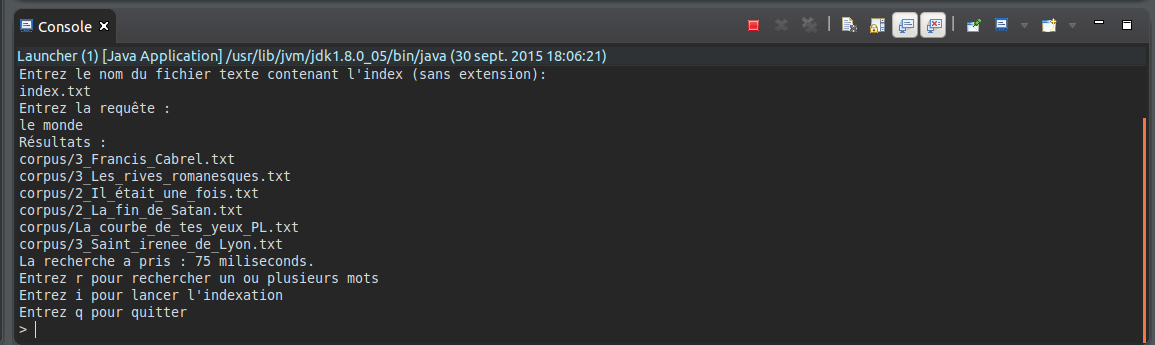
\includegraphics[scale=0.4]{../data/recherche.png}
\end{center}

\end{document}
